%%%%%%%% ICML 2025 EXAMPLE LATEX SUBMISSION FILE %%%%%%%%%%%%%%%%%

\documentclass{article}


\usepackage{fontspec}
\usepackage{newunicodechar} % 关键:用于字符映射
% 设置强大的字体回退链 (确保这些字体已安装)
\setmainfont{Times New Roman}  % Windows自带字体
% 设置Kannada字体 - Windows 8+ 自带Nirmala UI
\newfontface{\kannada}{Nirmala UI}

% 项目要求
% 1. 基础功能层(必须完成)
% –  集成至少1个大语言模型API(如GPT-3.5/4、qwen、deepseek等),展示不同参数(如temperature=0.7 vs 1.2)对输出的影响对比
% –  实现核心功能闭环,需定义明确的输入输出规范(如JSON Schema)并实现校验机制
% –  包含基础交互界面(命令行/CUI/GUI任选)√
% –  处理一些真实场景测试数据作为展示 √
% –  包含下方“技术实现规范”中的要点。
% 2. 进阶功能层(选择性完成)
% –  实现多模态扩展(图像/语音输入输出) x
% –  实现高质量结构化输出控制,能95%的概率生成符合要求的格式√
% –  构建领域知识库增强,如RAG架构需说明embedding模型选型(如text2vec)和检索策略(如FAISS索引)x
% –  开发记忆机制(对话历史/用户画像)√
% –  集成外部工具(包括但不限于计算器、数据库、API、Python代码解释器)x
% –  实现一个自主“Agent”,需实现至少3种工具调用决策逻辑 √
% –  其他可能的额外功能 √
% 3. 创新维度(选择性完成)
% –  解决未被主流产品覆盖的需求痛点
% –  提出新颖的prompt engineering方案
% –  设计独特的输出呈现形式
% –  其他可能的创新形式
%    注:以上括号内的,均是举例,而非必须和仅仅。比如集成的外部工具可以从括号中选几个,也可以自己再额外设计。

% 技术实现规范
% 1. 模型调用
% –  必须展示API调用参数调优过程(temperature/top_p等)
% –  需处理流式响应,实现逐字/分块输出效果(如ChatGPT式打字机效果),禁用单次完整响应√
% –  实现输入预处理(敏感词过滤/指令注入防护)【?】
% 2. 系统架构
% –  需提供架构设计图(数据流图/模块关系图)
% –  要求模块化开发(至少3个独立功能模块)√
% –  必须包含异常处理机制(API失败重试、结构化输出失败等)√

% Recommended, but optional, packages for figures and better typesetting:
\usepackage{microtype}
\usepackage{graphicx}
\usepackage{subfigure}
\usepackage{booktabs} % for professional tables
\usepackage{ctex}
\usepackage{float} %设置图片浮动位置的宏包

% hyperref makes hyperlinks in the resulting PDF.
% If your build breaks (sometimes temporarily if a hyperlink spans a page)
% please comment out the following usepackage line and replace
% \usepackage{icml2025} with \usepackage[nohyperref]{icml2025} above.
\usepackage{hyperref}



% Attempt to make hyperref and algorithmic work together better:
\newcommand{\theHalgorithm}{\arabic{algorithm}}

% Use the following line for the initial blind version submitted for review:
% \usepackage{icml2025}

% If accepted, instead use the following line for the camera-ready submission:
\usepackage[accepted]{icml2025}

% For theorems and such
\usepackage{amsmath}
\usepackage{amssymb}
\usepackage{mathtools}
\usepackage{amsthm}

% if you use cleveref..
\usepackage[capitalize,noabbrev]{cleveref}

%%%%%%%%%%%%%%%%%%%%%%%%%%%%%%%%
% THEOREMS
%%%%%%%%%%%%%%%%%%%%%%%%%%%%%%%%
\theoremstyle{plain}
\newtheorem{theorem}{Theorem}[section]
\newtheorem{proposition}[theorem]{Proposition}
\newtheorem{lemma}[theorem]{Lemma}
\newtheorem{corollary}[theorem]{Corollary}
\theoremstyle{definition}
\newtheorem{definition}[theorem]{Definition}
\newtheorem{assumption}[theorem]{Assumption}
\theoremstyle{remark}
\newtheorem{remark}[theorem]{Remark}

% Todonotes is useful during development; simply uncomment the next line
%    and comment out the line below the next line to turn off comments
%\usepackage[disable,textsize=tiny]{todonotes}
\usepackage[textsize=tiny]{todonotes}


% The \icmltitle you define below is probably too long as a header.
% Therefore, a short form for the running title is supplied here:
\icmltitlerunning{Submission and Formatting Instructions for ICML 2025}

\begin{document}

\twocolumn[
\icmltitle{人工智能基础 大作业报告}

%示例,根据自己的背景更改
\begin{icmlauthorlist}
\icmlauthor{陈凯丰}{2400934023}
\icmlauthor{李铭乐洋}{2400934034}
\icmlauthor{队员姓名3}{背景1}
\icmlauthor{队员姓名4}{背景2}
\icmlauthor{队员姓名5}{背景2}
\end{icmlauthorlist}


%示例,根据自己的背景更改
% \icmlaffiliation{背景1}{计算机学院, 北京大学, 年级}
% \icmlaffiliation{背景2}{环境学院, 北京大学, 年级}

% 显目关键词,根据自己的项目更改
\icmlkeywords{大模型,机器学习,命令行}

\vskip 0.3in
]

% 项目摘要
\begin{abstract}
很短的项目摘要
\end{abstract}

% 项目内容
\section{主题}

项目的主题和需求来自朱汶宣同学安装 Jupiter Notebook 的经历,由于一些依赖和 WSL 的问题,他希望能够有一款轻量级的产品能够帮助他定制化地精细分析运行命令过程中的问题。

随后我们将项目主题定为了 LLM 集成的轻量级终端。

\subsection{需求分析}

为了帮助用户解决在命令行下的问题,首先应当监控命令行的输出,然后在接到用户指令之后将这些信息处理并调用 LLM 获得建议,最后将建议呈现在用户界面上,供用户选择采用。并且,鉴于部署 github 仓库经常发生,于是也一并加上对各种项目部署的建议的生成。

我们决定将开发目标平台定在 windows 上,因为小组几位同学使用的都是 windows 电脑,并且 windows 原生的命令行生态并不成熟,相对于 Linux 和 Mac 缺少统一的管理器,遇到的环境和配置问题可能更多。

\subsection{技术选型}

为了能够在短时间内进行开发,我们小组决定使用 python 进行开发,优先采用已有的开源库来提高开发效率。

在查阅资料之后,我们决定使用 pywinpty 库来实现 windows 下和终端的交互,这个封装了系统调用,维护了一个伪终端(Pseudo Terminal)对象,使得程序可以和运行当中的命令行进行交互。

对于和 LLM 交互的部分,我们决定使用较为成熟的 openai 库来实现和远程 API 的交互。

由于实现一个 GUI 过于复杂,需要实现的终端渲染内容过多(如虚拟控制字符等),我们决定实现一个 CLI,直接利用 windows 已经实现好的终端应用(如 windows terminal 等)。

\subsubsection{总体架构}

项目总体包括如下模块:

\begin{itemize}
    \setlength{\itemsep}{0.1em}
    \setlength{\parskip}{0.1em}
    \item 模拟终端模块:封装和 shell 的交互。
    \item CLI 模块:实现用户交互,维护命令行历史内容。
    \item 记忆模块:实现和 LLM 交互的短期和长期记忆。
    \item LLM 模块:封装和 LLM 的交互。
    \item agent 模块:总结和处理信息,将上下文、记忆和问题交给 LLM 模块。
    \item 部署模块:针对部署项目(尤其 git 仓库)要求生成特别的部署计划。
    \item 安全模块:检测命令安全性。
    \item utils 模块:工具模块。
\end{itemize}

【这里需要插入一个图】

\subsubsection{模块简介}

CLI 模块是整个程序的入口以及交互界面,其中维护了一个内建的模拟终端对象和 Agent 对象,CLI 负责捕获用户的输出,判断是否是询问指令,并且将输入交给模拟终端或 Agent,同时异步地监听终端的输出。

utils 模块实现了一些独立的命令行工具和功能,如行内刷新输出等。

模拟终端模块实现了一个模拟终端类,在设定启动命令后异步地读取内建终端的输出,将输出异步地将输出回传给 CLI。

LLM 模块,封装了获取 API Key 已经和远端 API 的调用,以及从 LLM 中获取建议的 prompt engineering。

记忆模块(memory)封装了更新短,中和长期记忆的过程,以及总结生成新记忆的 prompt 工程。

安全模块(security)封装了对命令安全性的两步检验。

部署建议模块(deploy)封装了对于 github 仓库给用户提供部署建议的方法。

Agent 模块统筹规划了上述各个模块的工作,并在得到用户输入后进行调用。

上述中重要的模块将在实现细节中展开。

\subsection{实现细节}

\subsubsection{模拟终端和 CLI}

pywinpty 的伪终端支持向 stdin 写、从 stdout 阻塞地读。

windows 下的 shell(如 powershell)本身维护了一个缓冲区,接受用户输入的字符,包括可显示字符和不可见的控制字符,如 Ctrl-C、Backspace、左键等,并且实时向 stdout 输出带有控制台虚拟终端序列的 ANSI 字节流。

windows 下的终端,如 conhost、windows terminal、git bash 等均实现了控制台虚拟终端序列的控制和渲染,事实上每输入一个字符,windows 下的终端软件会接收到 shell 输出的 ANSI 字节流,要求软件重新渲染最后一行,以此达到动态输入的目的。因此直接捕获字符写入伪终端这可能导致大量重复的输出,为了解析这些输出需要较大的工作量。

为了解决这个问题,我们决定牺牲部分终端的便捷性,采用一次输入一行的方法,如此输入不会重复出现,虚拟终端序列的去除也较为方便,同时还能够直接利用 windows 下终端对 ANSI 字节流的支持。

因此启动 CLI 的主进程就是一个循环,阻塞地读取用户一行的输入,并且将其经过处理交给 Agent 或写入内建伪终端。

由于 shell 的输出时间并不规律,从内建伪终端的读取必须是异步的,模拟终端类中新建了一个进程进行读取和传回。在 CLI 中,一个回调函数被传递给模拟终端类,在读取到输入后将新输入的内容加到历史队列中并输出到用户界面上,其中数据结构的锁都由 python 内置库管理。

在用户输入调用 Agent 时,CLI 会将目前所有的历史记录和目录等信息传递给 Agent,Agent 经过处理以及和 LLM 的交互后返回一个命令列表,用户确认后在模拟终端中执行。

\subsubsection{Agent 实现}

Agent 是负责连接表面的和用户交互的 CLI,以及内部的需要利用语言模型的各个模块的枢纽。

在接受到普通命令时,CLI 会将命令发送给 Agent,Agent 将会将命令发送给记忆模块,更新记忆。

在接收到问询命令(即 ?? 开头的命令),CLI 会将该命令发送给 Agent,Agent 将调取记忆模块的所有记忆,并结合获取的环境信息,发送给 LLM 的 Handler,之后得到一个命令建议的列表,或者想要重新询问用户的请求,呈现给用户。若是重新询问用户的请求,则将不断重复上述的操作,直到用户选择退出,或者从 Handler 得到命令建议的列表。询问用户想要采取哪个方案后,Agent 会将该命令发送给安全模块,由安全模块做执行前的最后一次确认。确认完毕后,Agent 会将这个命令发送给 CLI 进行执行,并发送给记忆模块更新记忆。

在接收到部署建议(即 deploy 开头的命令),CLI 会将该命令发送给 Agent,Agent 会将该命令转发给部署建议模块,获取建议后呈现给用户。

\subsubsection{LLM 接口处理}

LLM\_core 中含有 API 密钥管理,LLM 调用函数以及流输出的函数。这几个函数都是平凡的。

API 密钥管理负责接收用户的 API,将其加密存储在文件系统中后,并在需要的时候返回。

LLM 调用则负责给定 prompt,向 LLM 获取回答。

流式输出则负责向命令行流式输出 LLM 的回答。

\subsubsection{Handler 与 Prompt 工程}

Handler 负责整理两个内容:整理各种信息并向 LLM 提问,以及根据格式解析 LLM 的返回结果。

Prompt 首先给出记忆与环境信息,然后给出用户的需求以及过往用户对 LLM 所提问题的回答,然后再向 LLM 描述任务以及格式要求。

由于我们需要 LLM 学会向用户提问,所以 Prompt 工程中强调了何时应当向用户提问,而何时应当用已知的信息直接给出回答:“...如果你没有收到请求,或者觉得用户用词模糊,或不足够清楚自己要做什么任务,或者在执行中遇到困难,或者遇到了未能处理的问题。请先返回一个'0',然后返回一个疑问句,即你的询问,然后不再给出任何内容!询问后也不用添加{\kannada{ಠ}}!否则先返回一个'1',然后给我提供若干可供接下来执行的选项。”

一个细节是,由于命令的特殊性(包含大量如反斜杠等字符),经过了多次测试,为了避免生成信息内容对解析的干扰,我们采用了以特殊字符'{\kannada{ಠ}}'作为分割符号来进行 Prompt 工程:“...选项不用太多,要求内容精简直接,数量最多五个。每一个选项的格式是三元组:该选项对应的可供执行的Powershell cmd命令(一定是能在终端执行的命令!){\kannada{ಠ}}该选项的说明{\kannada{ಠ}}该选项的注意事项{\kannada{ಠ}}。并且三元组都要给出内容,且以{\kannada{ಠ}}分隔,注意每一项后面都要加{\kannada{ಠ}}。”。采用此方案后,没有遇到过解析出错的情况。

在出现问题的情况,将抛出错误。用户再次输入 “??” 即可重试。

\subsubsection{安全检查}

当 Agent 决定直接执行某个语言模型获取的命令建议的时候,这个命令会发送给安全检查。安全检查模块负责二次判断语言模型给出 的命令是否有潜在的安全隐患。

安全检查采用两步的检查方案。第一步采用直接进行关键词检索,若命令不含有可能危险的关键词(如 rm 等),则直接通过安全检测。

未能通过第一步安全检查的命令,将询问语言模型该命令的安全性。若安全,则直接通过安全检测,否则将同时返回一个警告,告知用户该命令可能会产生什么样的潜在安全隐患。

\subsubsection{历史记忆与用户画像}

记忆模块维护了用户的短期记忆(近期的若干条命令),中期记忆(当前命令行的操作历史总结)与长期记忆(用户画像)。

每次用户进行命令的输入,Agent 都将会把命令发送给记忆模块,记忆模块将根据该命令更新三个记忆。

短期记忆将记录用户最近的若干条命令。

中期记忆:而对于提前设定好的 truncated 超参数 $\text{SHORT\_HISTORY}$(默认为 10),每隔这么多条消息之后,就将通过语言模型生成截至到目前为止的所有命令的总结,以节省记忆大小。

长期记忆:当用户关闭客户端,将调用记忆模块的长期记忆更新操作。记忆模块会利用语言模型,将之前的用户画像和此次命令行的中短期记忆进行总结,得到一份新的用户画像。用户画像包括了用户在命令行的行为习惯与偏好,熟悉程度,以及之前所在命令行做过的一些重要操作。

在需要的时候,记忆模块会将所有的记忆整合后发送给 Agent。

\subsubsection{部署建议模块}

部署模块的 deploy 功能分为两种。当 deploy 的内容并非 github 仓库,则直接尝试通过问询语言模型,用语言模型本身的知识库获取部署的方案。

否则,若接收的是一个 github 仓库的 url,通过访问该 url 拉取仓库中的 readme 后。随后,函数将结合用户记忆以及环境信息,向语言模型索取部署建议。

语言模型将分析该 readme 中是否含有部署信息,或者对于较为知名的项目,动用本身的知识给出部署的建议方案。由于多数情况下 readme 中含有的信息不足以直接给出若干个命令,故仅返回较为具体的部署方式,由用户自己进行执行。

部署建议为一个有序列表,返回给 Agent。

\subsubsection{模型选择}

考虑在不同的使用场景,对语言模型的精度,速度,推理能力等有不同的需求,故使用了不同的语言模型。

命令建议:获取建议的命令操作时,使用 DeepSeek-R1。这是因为该步骤对输出格式的要求较高且较复杂,并且命令可能较为复杂,需要足够准确。所提供的信息(如过往的记忆,用户的想法等)较多,需要一定的推理能力。

安全模块:在安全模块的第二次检验中,使用 Qwen2.5-7B-Instruct。这是因为判断命令是否足够安全的任务简单,所输出的格式要求简单,在这一步采用更小的模型,减少用户在已知应该使用什么命令的情况下的等待时间。

记忆模块:在记忆模块的所有语言模型均使用 Qwen2.5-7B-Instruct。这是因为中长期记忆并不需要完全准确细致地进行总结,只需记录下用户做了些什么。并且当 $\text{SHORT\_HISTORY}$ 较小时,中期记忆可能会造成平凡的“卡顿”现象,使用更快的语言模型有助于缓解卡顿时间。

部署模块:部署模块调用 DeepSeek-R1。这是因为 README 文件可能较长,需要较好的文本理解与推理能力才能找到有用信息。

\subsubsection{参数调优}

在实现中模型由 topk 改动不明显与 temperature 的改动。因此我们主要进行了关于 temperature 的参数调优,而将 topk 固定为一个中性值 0.5 。

对于解决用户个性化问题的模块,temperature 高时(如 1.2)给出的回答会较为丰富,且更加的有想象力。temperature 低时(如 0.3)给出的回答会较为平凡且严肃,缺乏创造力。因此对于该项功能,使用较高的 temperature 会让模型有更好的表现。

对于 deploy 模块,temperature 无论高低,给出的回答都满足了需求的准确性。不过高 temperature 模型给出的回答用的文字数量明显更多,低 temperature 模型的回答更为简洁。因此对于该项功能,使用较低的 temperature 给出一个“严肃”的模型会更好。

在 vanilla version 中,我们统一将 temperature 设为一个中性值 0.7 。这是可以按照功能模块个性化定制的,不过既然 deploy 的准确性表现几乎无关 temperature,选定一个统一的值也是合理的。

在附录 A.1 中罗列了调优证据以及对它们的观察与总结。

\subsection{评估对比}

% 好像最近有个开源项目叫 fuck,大概就是 fuck 以下就可以修正上一条命令的错误,但那个是基于本地匹配规则的,这一点可以写一写。

\subsection{反思}

\subsubsection{项目要求对照}

在与项目要求进行检查的过程中,由于该项目的特殊性,有两个基础要求我们认为并不适用于此项目:


\begin{itemize}
\item “实现核心功能闭环,需定义明确的输入输出规范并实现校验机制”。由于命令行的特殊性,不符合输入规范的命令将直接由命令行返回错误信息,这也符合用户在日常使用中的习惯。在已有足够完善的命令行自带的规范的情况下,我们认为额外引入除了 “??” 和 “deploy” 之外的其他特殊的规范不会起到积极的作用。

\item “实现输入预处理(敏感词过滤/指令注入防护)”。除去对用户输入命令的解析,我们并未做敏感词过滤等等其他的非平凡的预处理。这是因为我们希望至少用户能将其作为一个正常的命令行使用,并且用语言模型减少其使用门槛,而并非通过各种方式减少用户命令的自由度。
\end{itemize}

\bibliography{example_paper}
\bibliographystyle{icml2025}


%%%%%%%%%%%%%%%%%%%%%%%%%%%%%%%%%%%%%%%%%%%%%%%%%%%%%%%%%%%%%%%%%%%%%%%%%%%%%%%
%%%%%%%%%%%%%%%%%%%%%%%%%%%%%%%%%%%%%%%%%%%%%%%%%%%%%%%%%%%%%%%%%%%%%%%%%%%%%%%
% APPENDIX
%%%%%%%%%%%%%%%%%%%%%%%%%%%%%%%%%%%%%%%%%%%%%%%%%%%%%%%%%%%%%%%%%%%%%%%%%%%%%%%
%%%%%%%%%%%%%%%%%%%%%%%%%%%%%%%%%%%%%%%%%%%%%%%%%%%%%%%%%%%%%%%%%%%%%%%%%%%%%%%
\newpage
\appendix
\onecolumn
\section{附录}

% 可以将一些额外的内容放在这里
%%%%%%%%%%%%%%%%%%%%%%%%%%%%%%%%%%%%%%%%%%%%%%%%%%%%%%%%%%%%%%%%%%%%%%%%%%%%%%%
%%%%%%%%%%%%%%%%%%%%%%%%%%%%%%%%%%%%%%%%%%%%%%%%%%%%%%%%%%%%%%%%%%%%%%%%%%%%%%%

\subsection{temperature 调优证据展示}

对于解决用户个性化问题的模块,我们采取了极端温度(1.2 / 0.3 / 0.05)以固定问题分别得到了两组回答(每组独立清空 memory)。

\begin{figure}[H]
\centering
\subfigure[result 1]{
\label{Fig.sub.1}
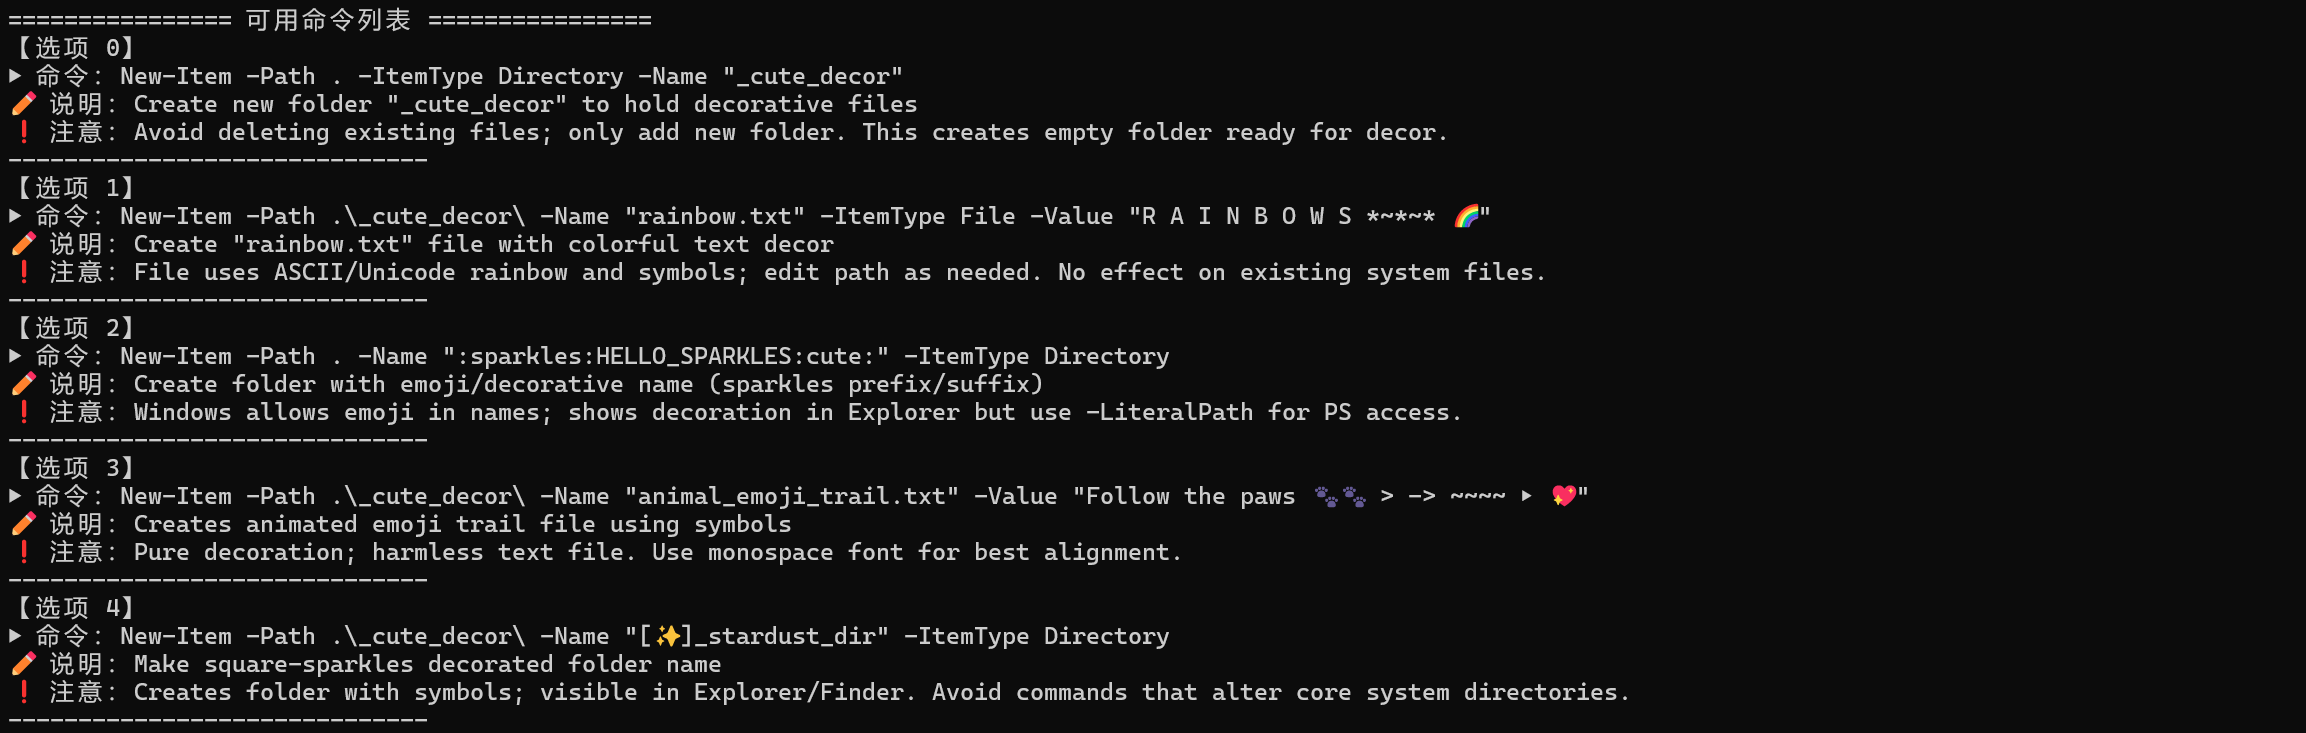
\includegraphics[width=0.45\textwidth]{img_q/1.2 & 0.5 (1).png}}
\subfigure[result 2]{
\label{Fig.sub.2}
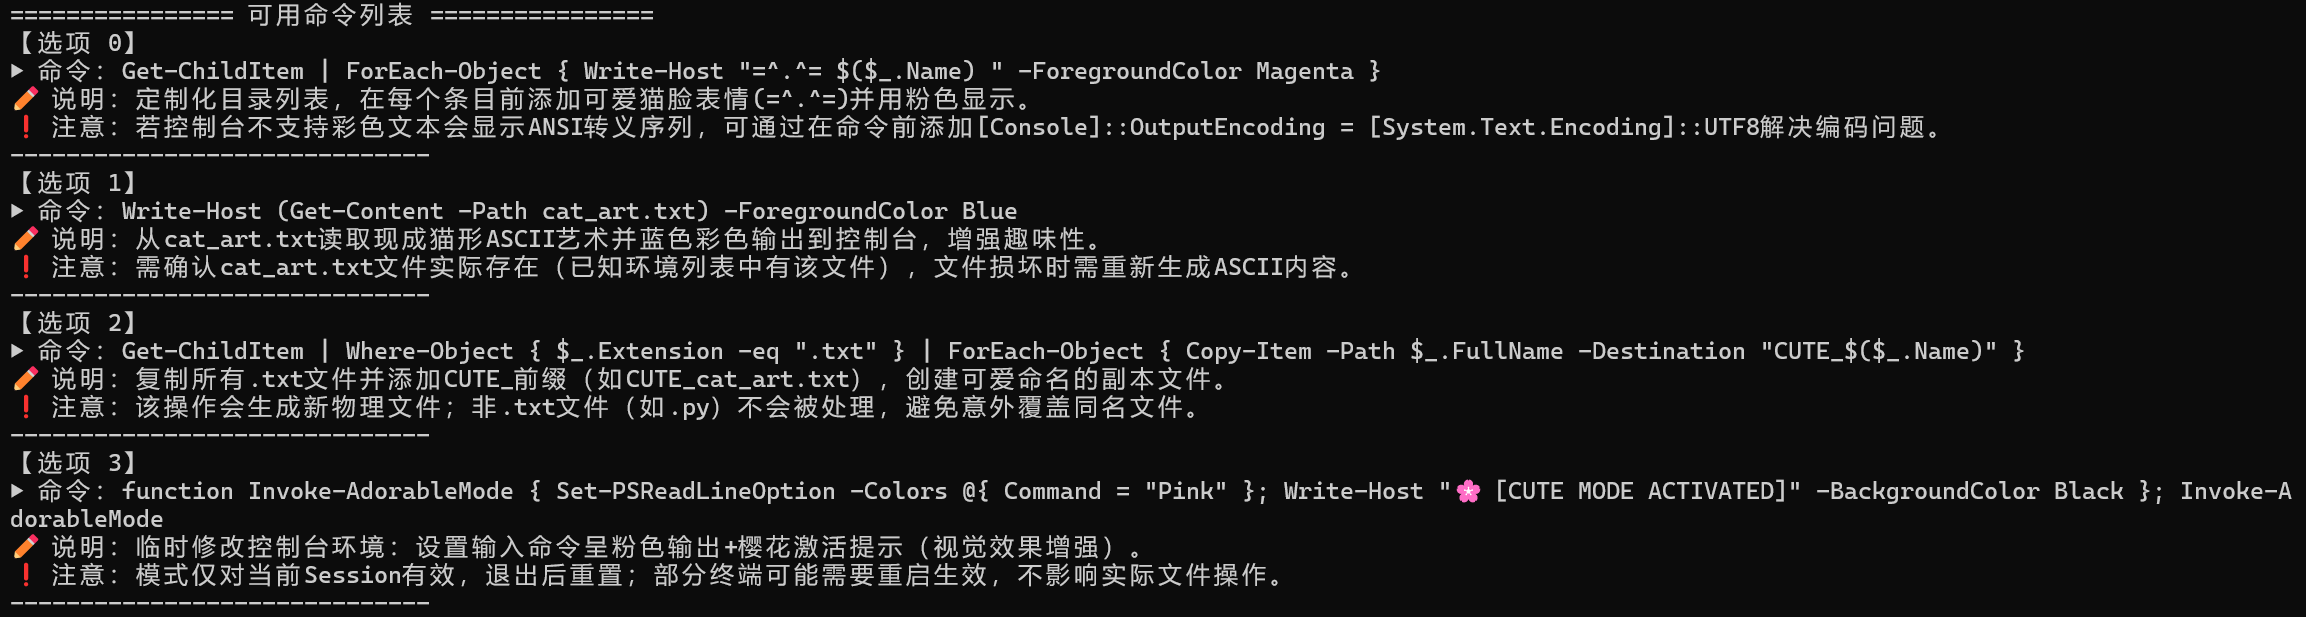
\includegraphics[width=0.45\textwidth]{img_q/1.2 & 0.5 (2).png}}
\caption{When the temperature is 1.2}
\label{Fig.main}
\end{figure}

相对来说 1.2 给出了较为创造性的提议,但下面两则就显得有些“无聊”:

\begin{figure}[H]
\centering
\subfigure[result 1]{
\label{Fig.sub.1}
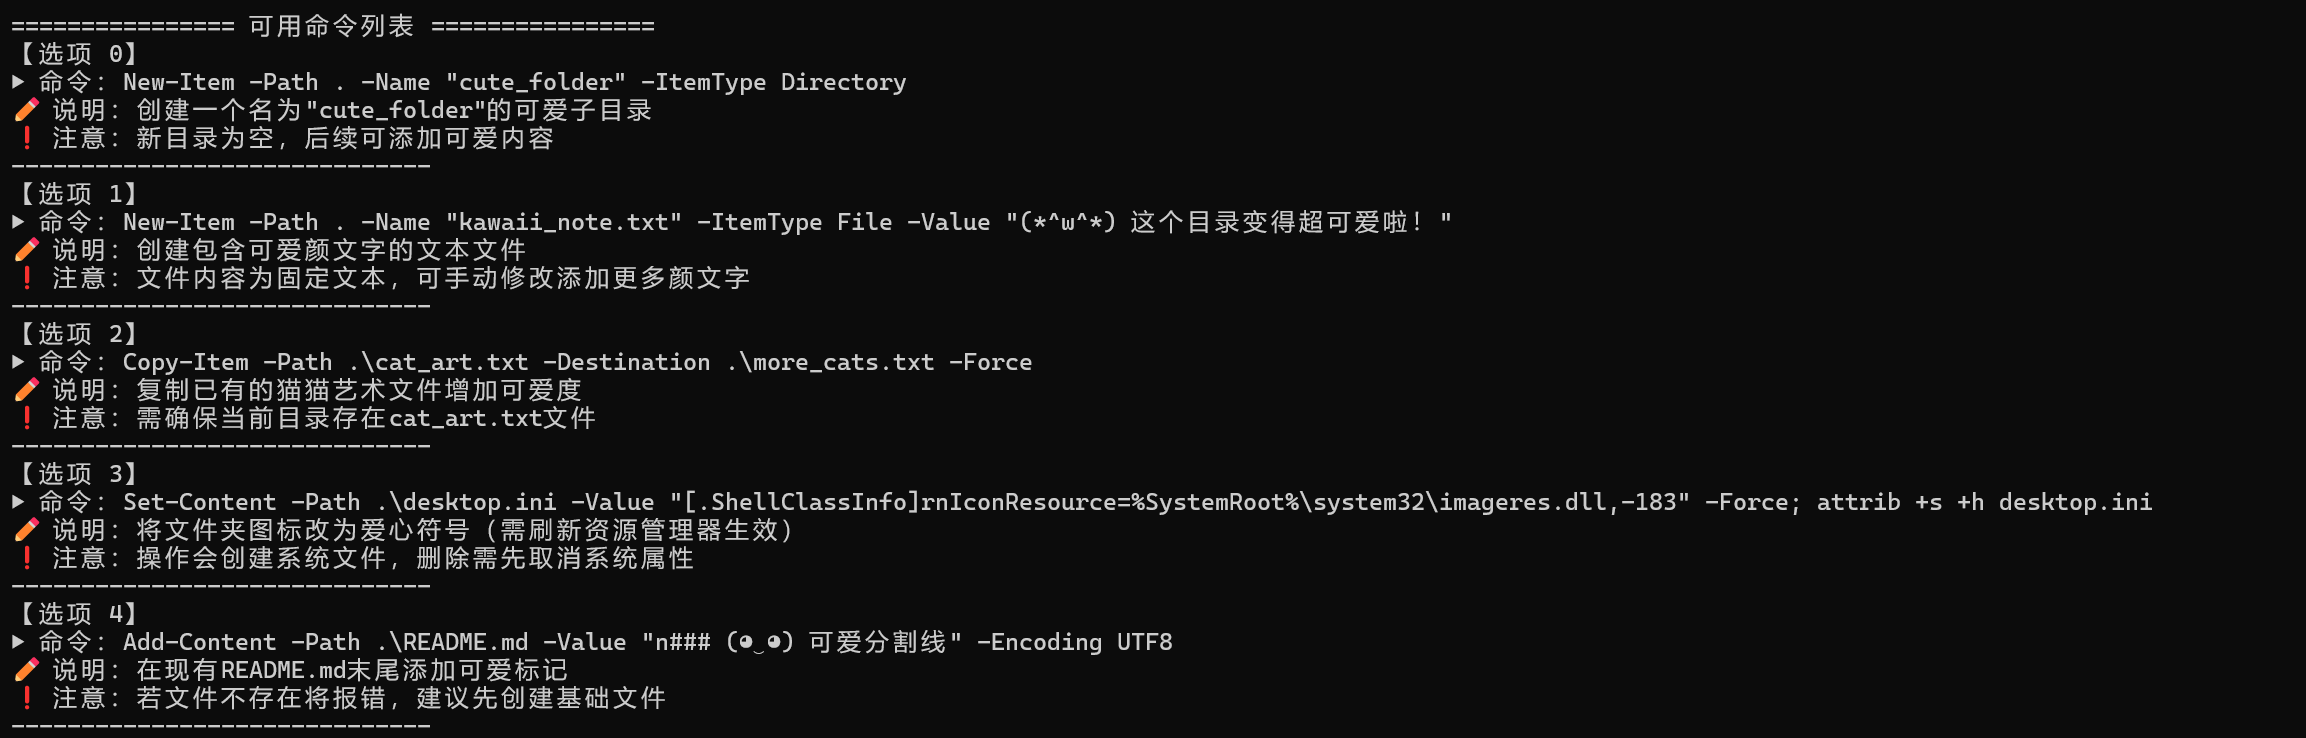
\includegraphics[width=0.45\textwidth]{img_q/0.3 & 0.5 (1).png}}
\subfigure[result 2]{
\label{Fig.sub.2}
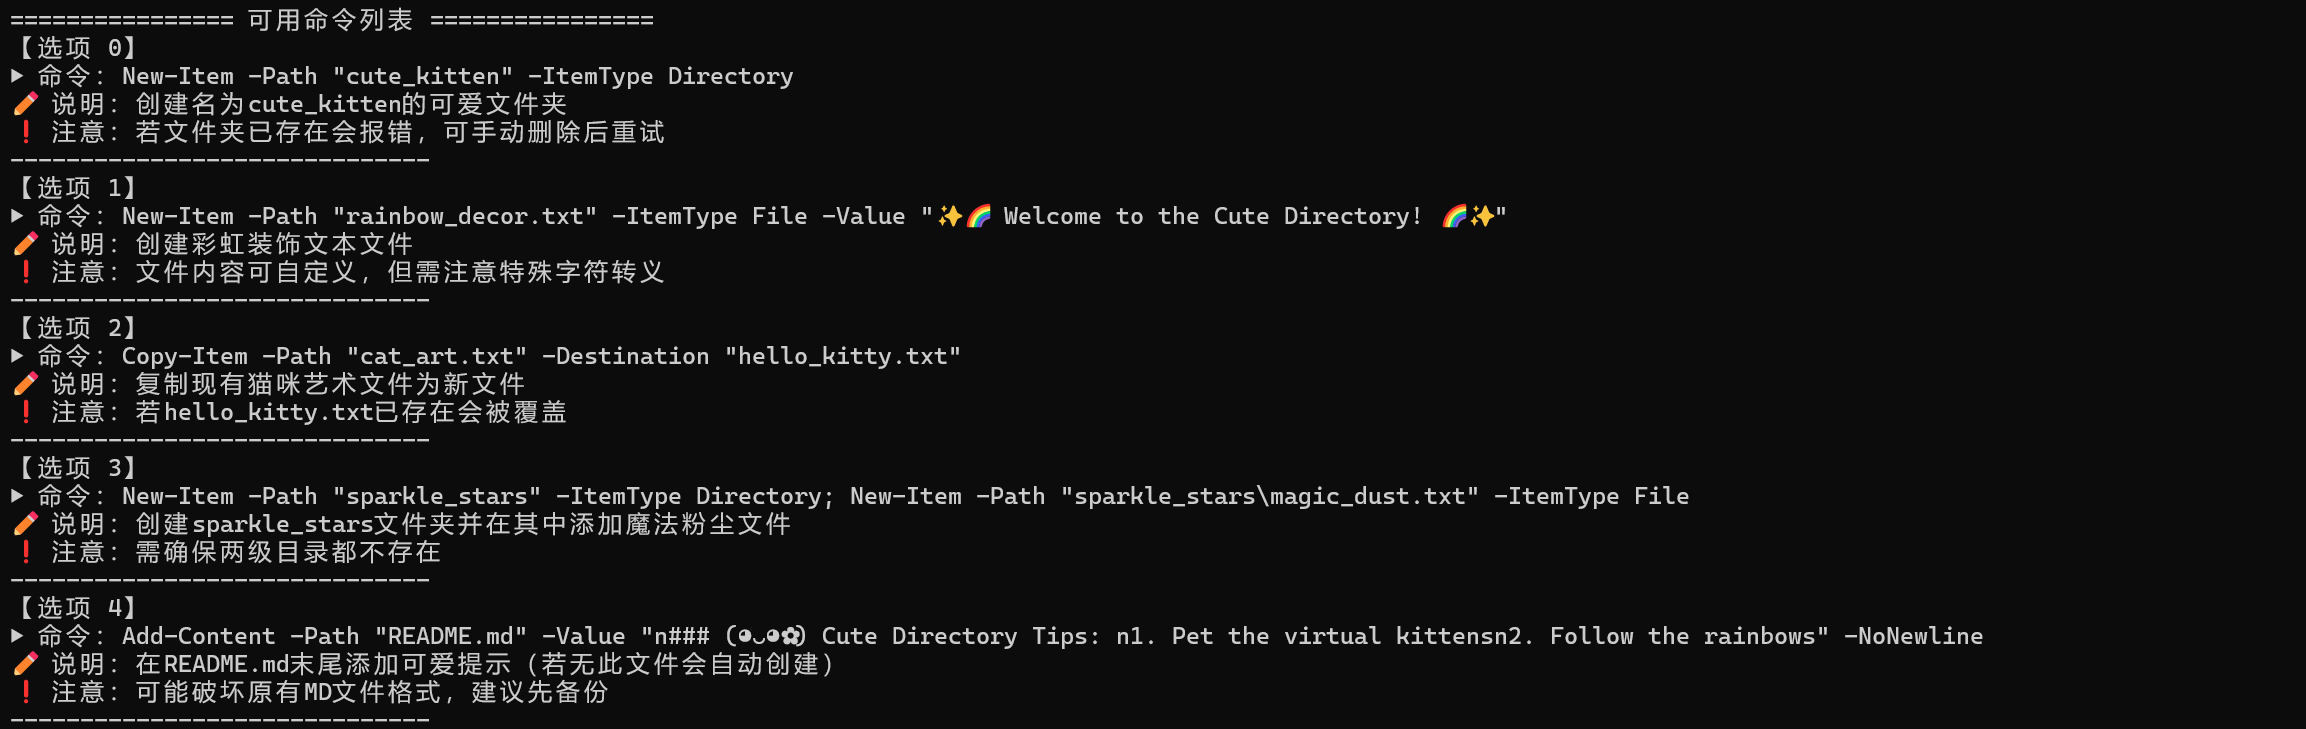
\includegraphics[width=0.45\textwidth]{img_q/0.3 & 0.5 (2).png}}
\caption{When the temperature is 0.3}
\label{Fig.main}
\end{figure}

\begin{figure}[H]
\centering
\subfigure[result 1]{
\label{Fig.sub.1}
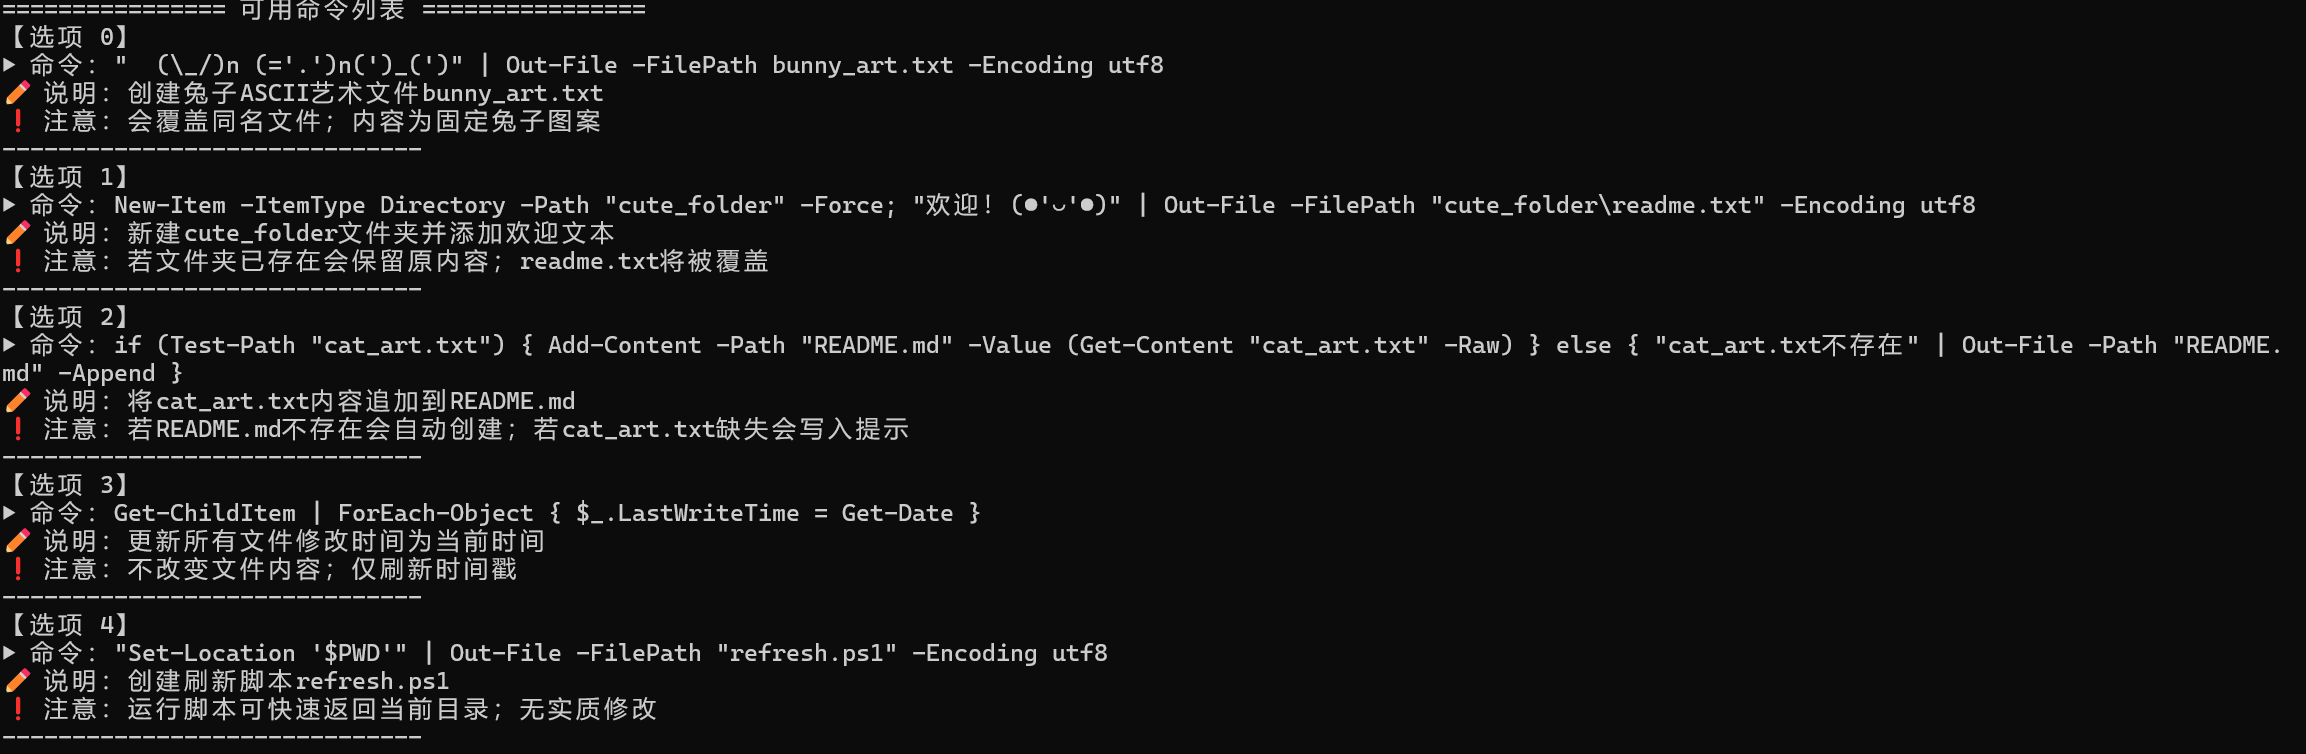
\includegraphics[width=0.45\textwidth]{img_q/0.05 & 0.5 (1).png}}
\subfigure[result 2]{
\label{Fig.sub.2}
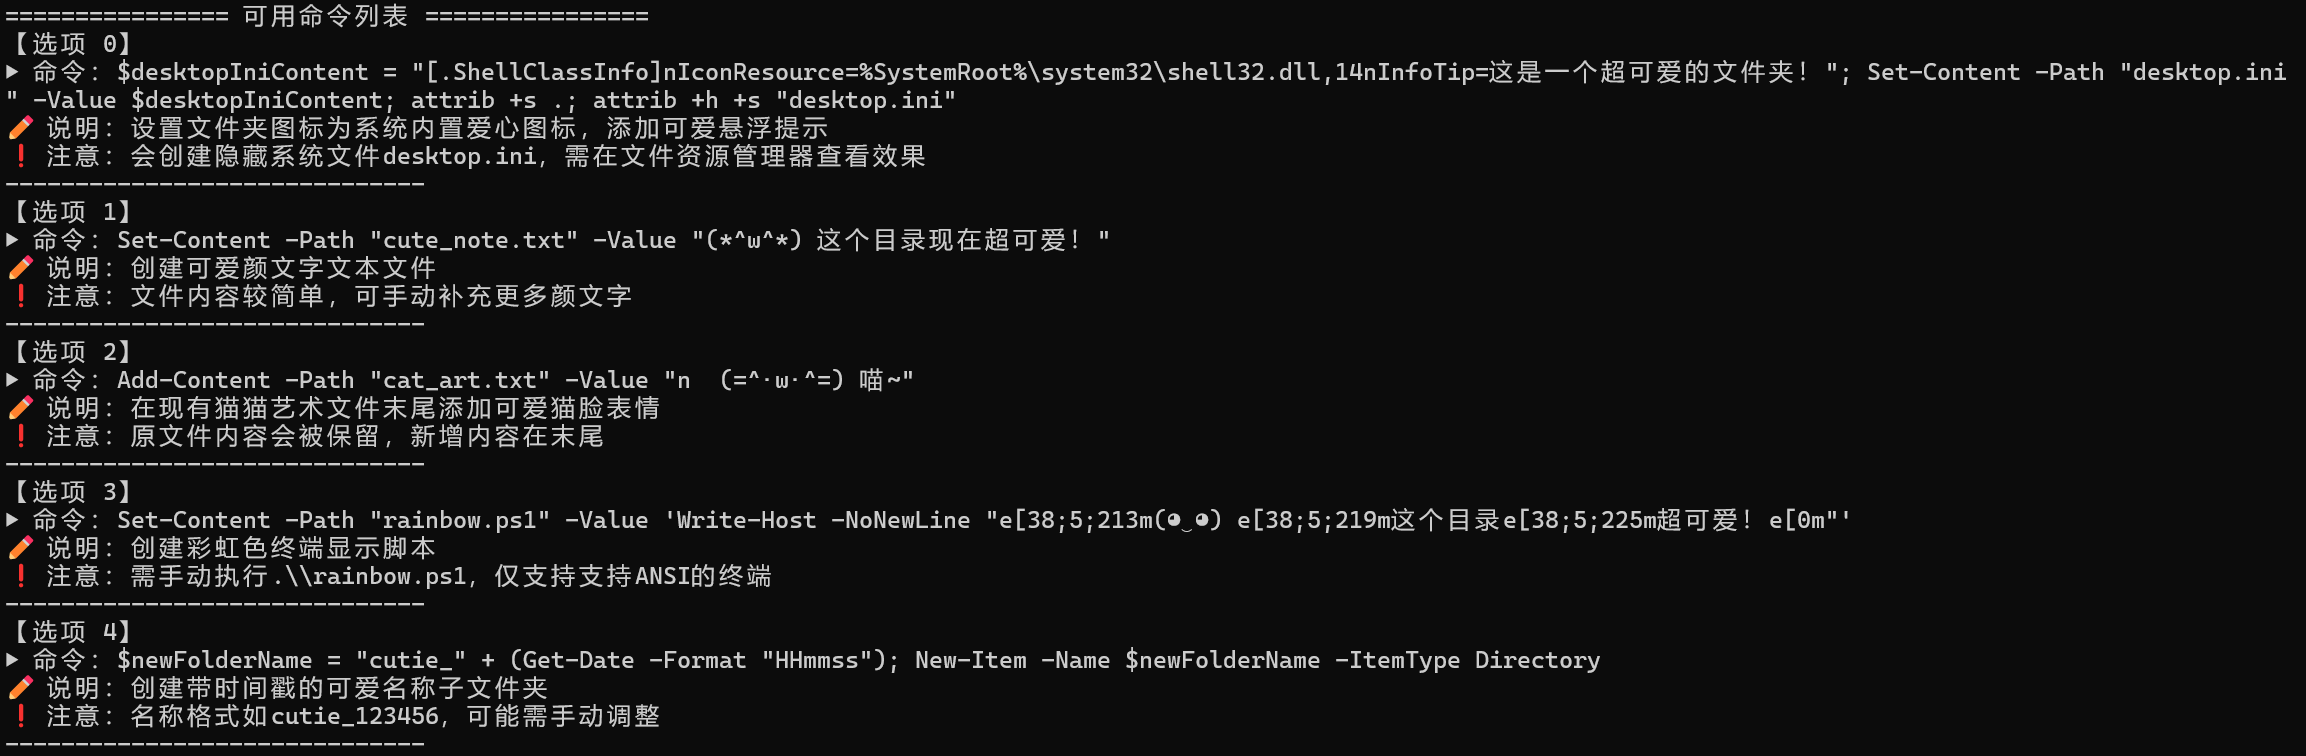
\includegraphics[width=0.45\textwidth]{img_q/0.05 & 0.5 (2).png}}
\caption{When the temperature is 0.05}
\label{Fig.main}
\end{figure}

对于 deploy 模块,由于大部分(著名)项目的部署都较为复杂,因此模型以给出建议为主。我们以 Flask(即 pallets/flask)和 GarmentPile(即 AlwaySleepy/Garment-Pile) 为例,展示所观察到的现象:

\begin{figure}[H]
\centering
\subfigure[0.2]{
\label{Fig.sub.1}
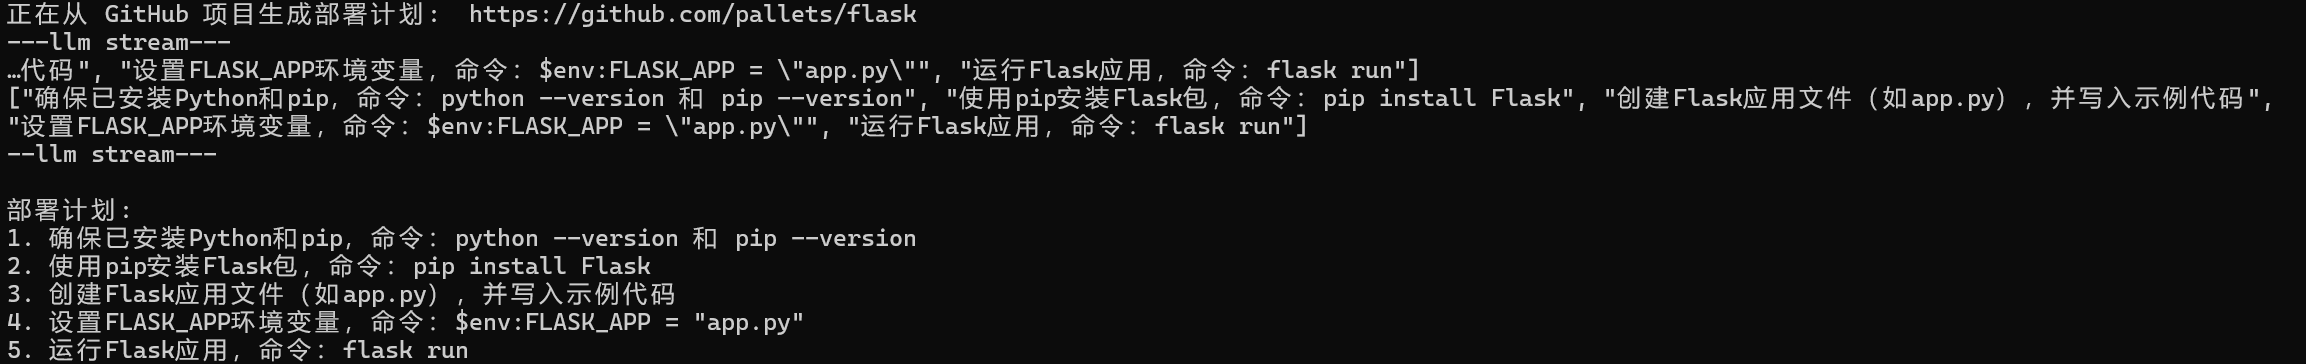
\includegraphics[width=0.45\textwidth]{img_d/flask_0.2.png}}
\subfigure[1.2]{
\label{Fig.sub.2}
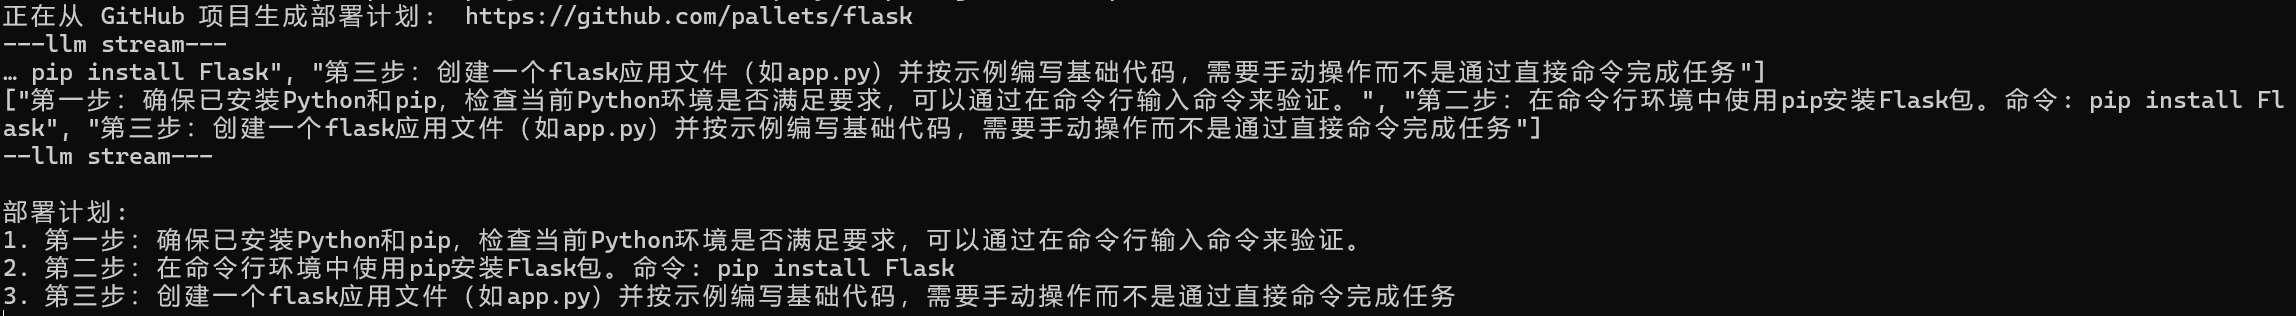
\includegraphics[width=0.45\textwidth]{img_d/flask_1.2.png}}
\caption{https://github.com/pallets/flask}
\label{Fig.main}
\end{figure}

\begin{figure}[H]
\centering
\subfigure[0.2]{
\label{Fig.sub.1}
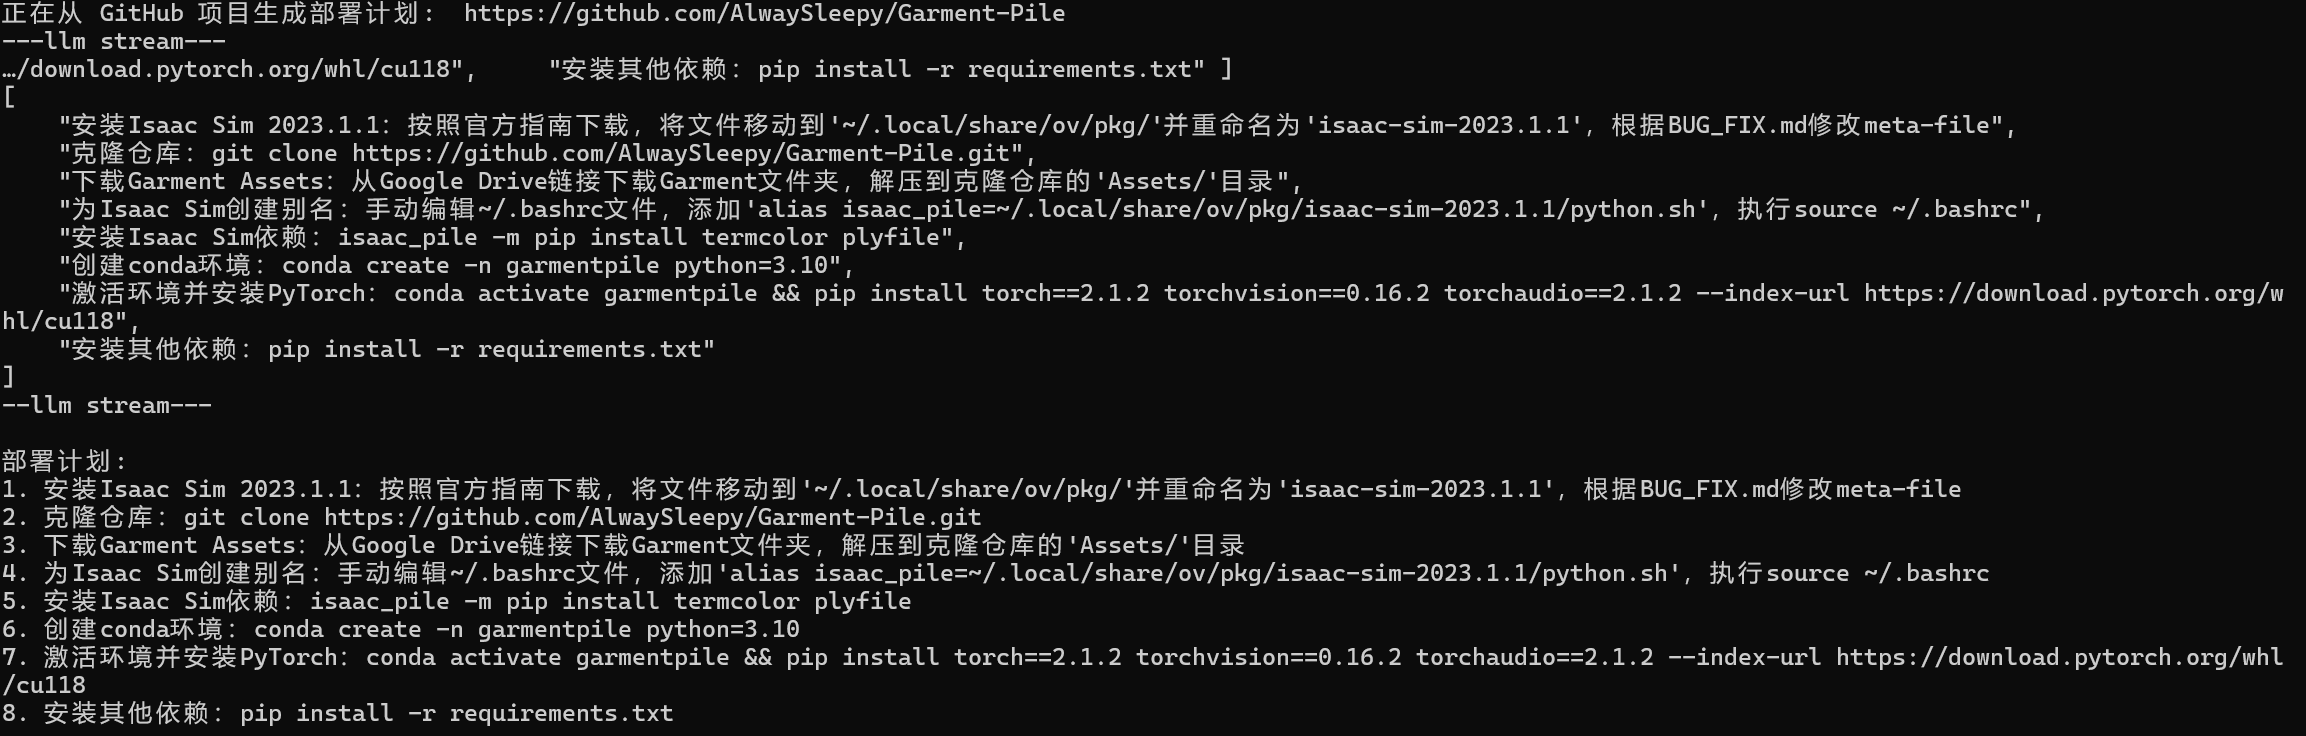
\includegraphics[width=0.45\textwidth]{img_d/gp_0.2.png}}
\subfigure[1.2]{
\label{Fig.sub.2}
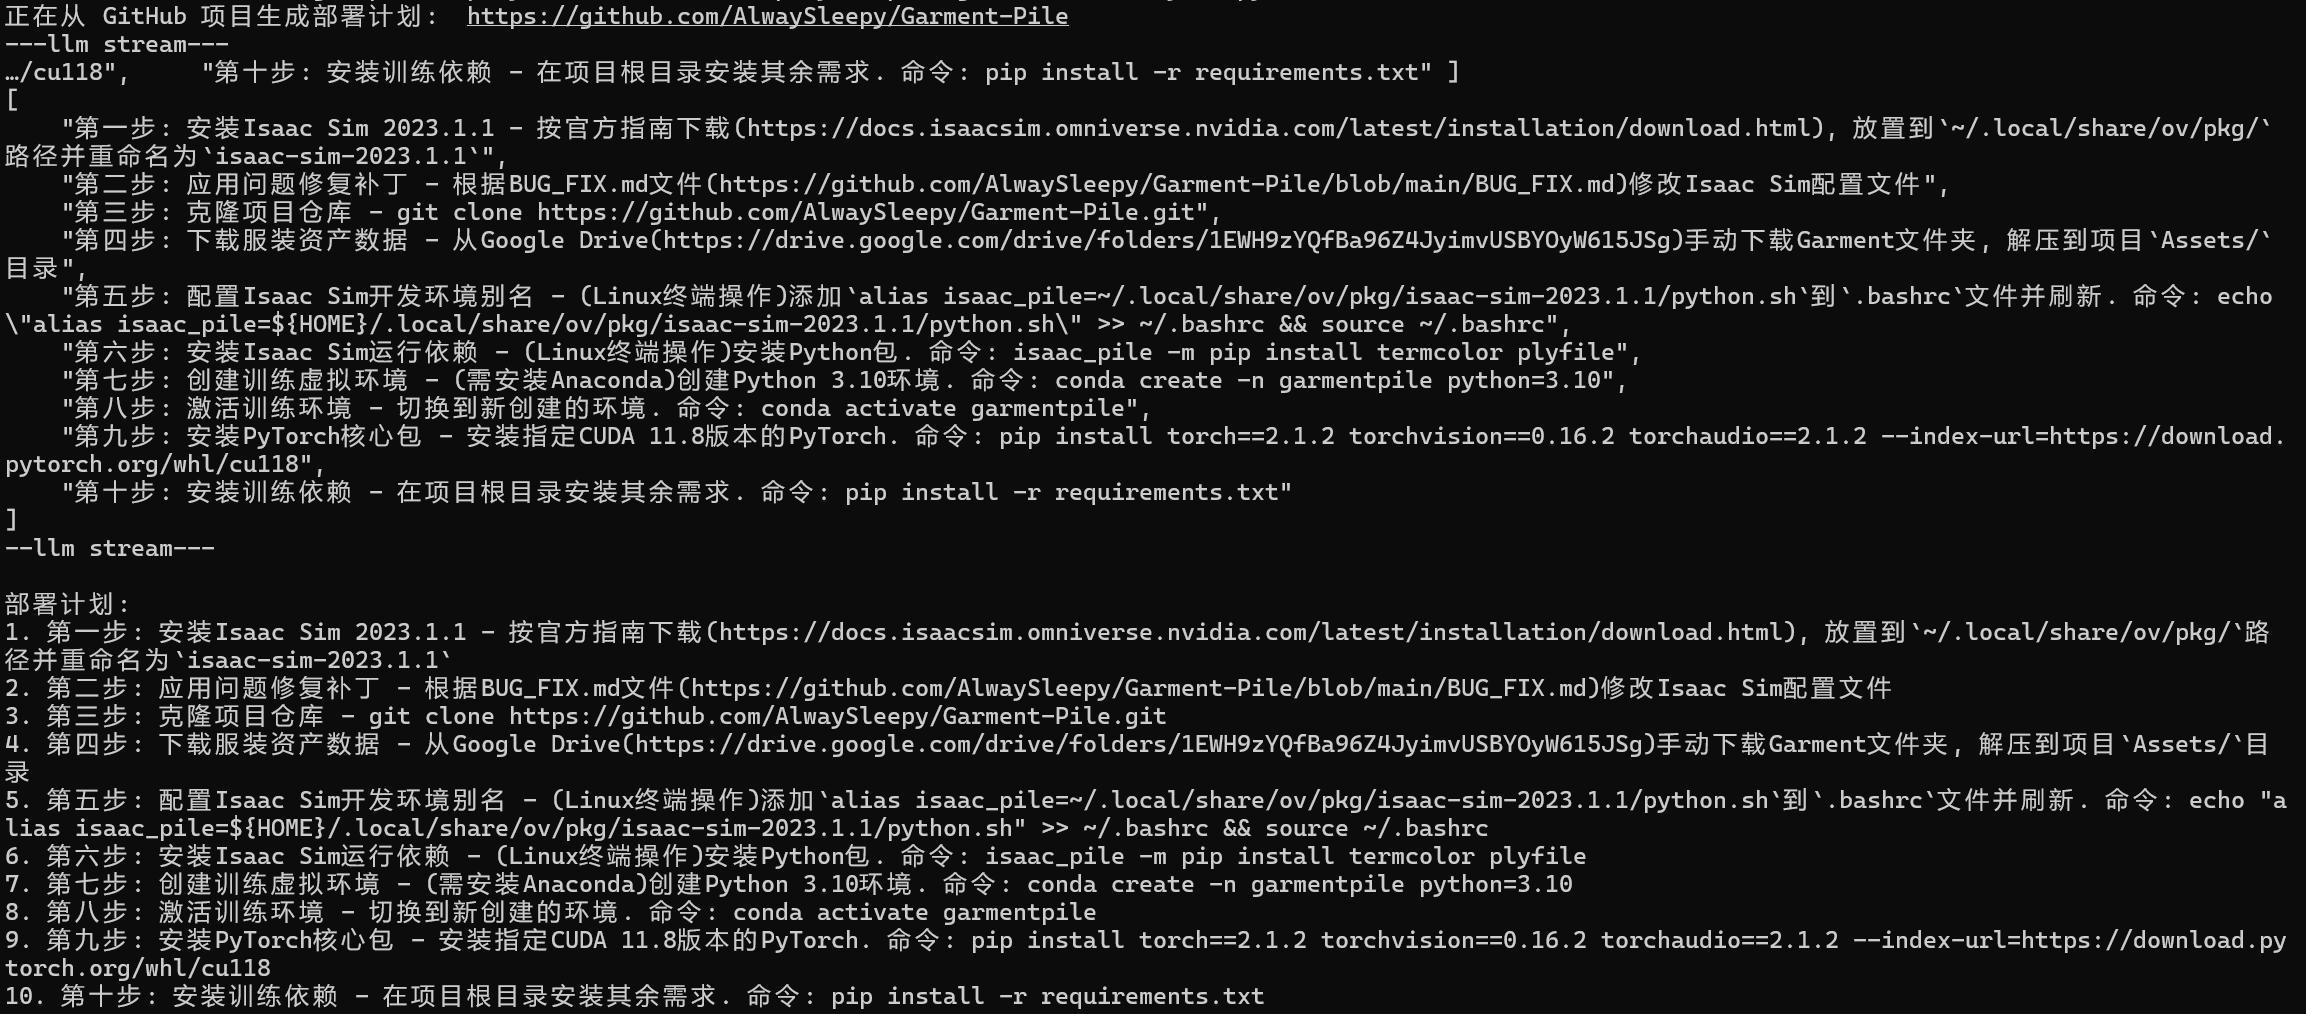
\includegraphics[width=0.45\textwidth]{img_d/gp_1.2.png}}
\caption{https://github.com/AlwaySleepy/Garment-Pile}
\label{Fig.main}
\end{figure}

两例的左图为 temperature=0.2 时的情况,右侧即为 1.2 。可以明显看到左侧较于右侧明显更为“严肃”。

\end{document}

%This document was modified from the file originally made available by
% Pat Langley and Andrea Danyluk for ICML-2K. This version was created
% by Shui Jie in 2025

